\section{Microverification}

The numerical material is a consistency check designed to falsify implementation or algebraic errors in the stated minimal model. It is \emph{not} empirical validation of the HLS programme.

The symbolic Jacobian audit reproduces Equation~\eqref{eq:beta-critical}. For $(\eta,\delta)=(0.4,0.2)$, it gives $c^*=0.5$ and $\beta_c=2$. Below the threshold, perturbed trajectories return to the symmetric state. At the threshold, the assignment mode is marginal and finite-horizon relaxation is slow. Above the threshold, the chosen symmetric parameterisation yields opposite polarized outcomes for positive and negative perturbations (Figure~\ref{fig:specialization}). This is \textbf{NUMERICALLY-VERIFIED} for this implementation and parameter setting only.

\begin{figure}[t]
\centering
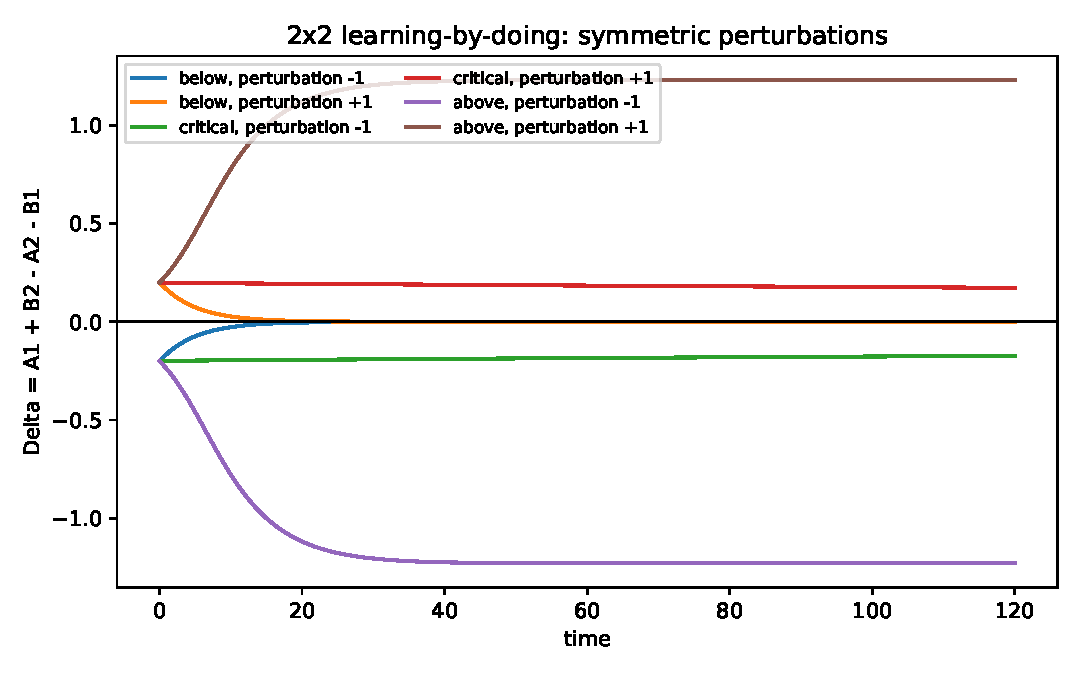
\includegraphics[width=0.82\linewidth]{../results/microverification/specialization_dynamics.pdf}
\caption{Diagnostic trajectories of the assignment gap in the symmetric learning-by-doing model. They verify the local-threshold calculation for one parameterisation; they are not empirical evidence of real HLS specialization.}
\label{fig:specialization}
\end{figure}

For CR1, $(\Delta_0,x,y)=(1,0.6,0.6)$ gives $G(x,0)=G(0,y)=0$ and $G(x,y)=0.2$. For CR4, an independent grid argmin matches Equation~\eqref{eq:rebalancing-solution} across TRAIN, boundary, MIXED, ROUTE, and selected limiting cases. The interior example $(d_0,a,v,g)=(1,1.5,1,1)$ yields $(x^*,y^*)=(0.5,0.5)$ and $Q_M=1.375<Q_T=Q_R=1.5$ (Figure~\ref{fig:rebalancing}).

\begin{figure}[t]
\centering
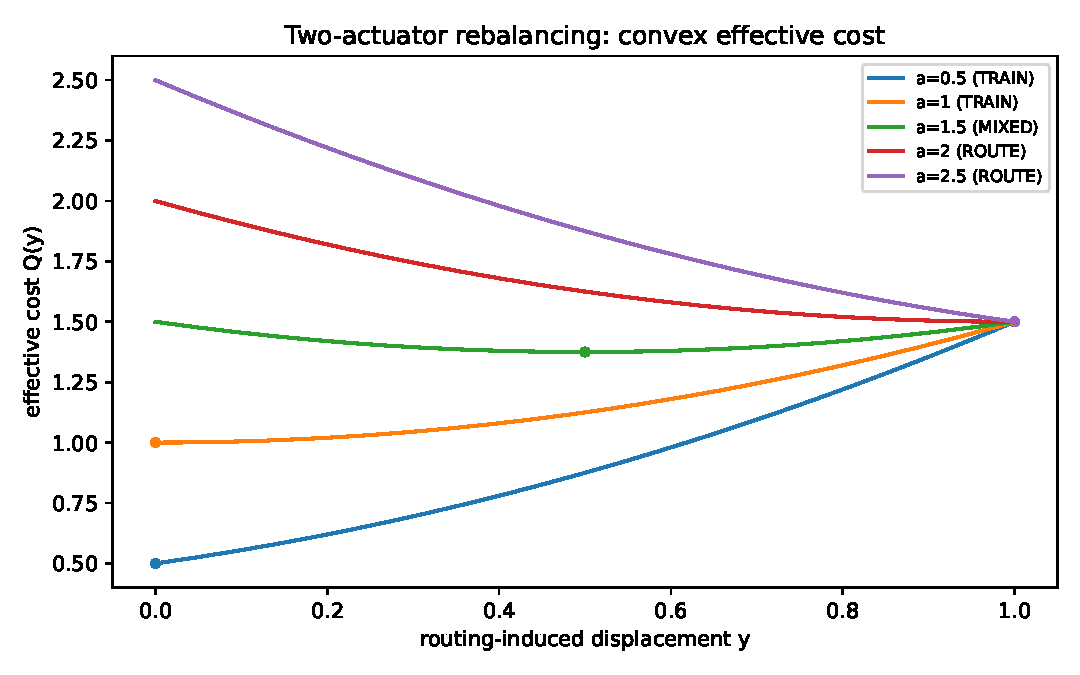
\includegraphics[width=0.82\linewidth]{../results/microverification/rebalancing_costs.pdf}
\caption{Diagnostic convex effective-cost curves for the two-actuator rebalancing calculation. The plotted parameter choices illustrate the closed-form TRAIN/MIXED/ROUTE regimes only.}
\label{fig:rebalancing}
\end{figure}
